\documentclass[12pt,a4paper]{article}

\usepackage{alltt}
\usepackage[utf8]{inputenc}
\usepackage[english]{babel}
\usepackage{amsmath}
\usepackage{amsfonts}
\usepackage{amssymb}
\usepackage{indentfirst}
\usepackage{setspace}
\usepackage[pdftex]{graphicx}
\usepackage{caption}
\usepackage{subcaption}
\usepackage{textcomp}
\usepackage{array}
\usepackage{listings}
\usepackage{color}
\usepackage{tikz} % для создания иллюстраций
\usepackage{hyperref}

\newcommand{\infers}{\,\to\,}
\newcommand{\tinfers}{\;\Rightarrow\;}

%\voffset = -118pt
%\textheight = 820pt
%\hoffset = -100pt
%\textwidth = 550pt
\newcommand{\htext}{0.46\textwidth}
\newcommand{\hstext}{0.45\textwidth}

\newcommand{\mat}[1]{\vec{#1}}
\newcommand{\framed}[1]{\tikz[baseline=(char.base)]{\node[shape=rectangle,draw,inner sep=4pt] (char) {#1};}}

%opening
\title{}
\author{}

\begin{document}


% TEAM.
\parbox{0.333\textwidth}{
	Maksim Velikanov \\[0mm]
}
% In der Mitte der Name der Veranstaltung.
\parbox{0.333\textwidth}{\vspace*{1mm}\begin{center}\large\bf%
		HPC with C++\\[0mm]
		SS 24\\[0mm]
\end{center}}
\parbox{0.333\textwidth}{
	\begin{flushright}
		Project report\\[0mm]
		17.02.2025\\[0mm]
	\end{flushright}
}
\par\vspace{-5mm}
\definecolor{freiburg-gray}{rgb}{0.68,0.68,0.68}
\vspace*{2mm}
\raisebox{1.19cm}{%
	\textcolor{freiburg-gray}{\rule{\textwidth}{1.1mm}}}

\bigskip




\section{Introduction}

In this project I implemented a Molecular Dynamics simulation in C++ consisting of individual atoms, based on the physics equations for interaction between atoms. The implemented program contains several experiments for testing and analysis of the simulation: generating a cubic lattice or using a precomputed icosahedron cluster; controlling the temperature of the simulation with a thermostat to prevent vaporization; monitoring the potential and kinetic energies; saving the atom positions to a file and visualization; heating the cluster and measuring the melting point and latent heat; running parallel simulation with OpenMPI; stretching a golden whisker and measuring stress.

The theoretical base is present in \hyperref[methods]{methods}, the details of implementation and results in \hyperref[experiments]{experiments}, and \hyperref[conclusion]{conclusion} at the end.

\section{Methods}
\label{methods}

The key methods for modeling a physical system of atoms are following:

\begin{enumerate}
	\item Update atom position and velocity, given constant force for a small time step --- {\bf Velocity-Verlet integrator}
	\item Estimate force between particles from the potential energy --- {\bf Lennard-Jones potential}
	\item Stabilization of the system by connecting it to a constant-temperature heat bath --- {\bf Berendsen Thermostat}
	\item Physically accurate N-body potential for modeling metals --- {\bf Embedded Atom Method potential}
	\item {\bf Domain decomposition} and parallel execution with OpenMPI
	\item Application of an external force --- {\bf Stress estimation}
\end{enumerate}

\newpage
\subsection*{Velocity-Verlet integrator}

The atom movement is approximated by assuming constant force and making small time steps. The method was rediscovered by Loup Verlet \cite{verlet} for Molecular Dynamics simulation.

Vector form of Newton's law gives:
\[ \dot{\mat{v}}_i(t) = \cfrac{\mat{f}_i(t)}{m_i} \]

Definition of velocity:
\[ \dot{\mat{r}}_i(t) = \mat{v}_i(t) \]

From these two formulas we get the approximation equations using Taylor formula.
Integration, predictor step:
\[
v_i(t + \Delta t/2) = v_i(t) + \cfrac{1}{2m_i} f_i(t) \Delta t
\]
\[ r_i(t+\Delta t) = r_i(t) + v_i(t+ \Delta t/2) \Delta t \]

After this step we must recompute the forces for new positions of atoms. Corrector step:
\[ v_i(t+\Delta t) = v_i(t+\Delta t/2) + \cfrac{1}{2m_i}f_i(t+\Delta t) \Delta t \]

\subsection*{Lennard Jones potential}

Here we derive a formula to compute the force from potential energy. By definition of pair potential:
\[
E_{pot} = \sum_{i<j} V(r_{ij})
\]

Lennard-Jones potential \cite{lennard-jones} is sum of Pauli Repulsion (repulsive force) and London Dispersion (attractive force). These interactions act even on uncharged atoms.

\[
V_{ij}(r) = 4\epsilon \left( \Bigl(\cfrac{\sigma}{r}\Bigr)^{12} - \Bigl(\cfrac{\sigma}{r}\Bigr)^{6} \right)
\]

By definition of energy, force is the derivative of energy by position.
\[
\mat{f}_k = \left( \begin{aligned}
	& - \partial E / \partial x_k \\
	& - \partial E / \partial y_k \\
	& - \partial E / \partial z_k \\
\end{aligned} \right) = \sum_i \cfrac{\partial V}{\partial r_{ik}} {\hat r_{ik}} \text{\ (unit vector)}
\]

Let's compute for one of the dimensions.
\[
\cfrac{\partial V_{ij}}{\partial x_k} = \text{(chain rule by vector length)} \cfrac{\partial V_{ij}}{\partial r_{ij}} \cfrac{\partial r_{ij}}{\partial x_k}
\]

\[ \cfrac{\partial r_{ij}}{\partial x_k} = \cfrac{\partial \sqrt{(x_j-x_i)^2 + \ldots}}{\partial x_k} = (*) \]
Remember: \( (\sqrt{u})' = \cfrac{1}{2\sqrt{u}} u' \)

\[
(*) = \cfrac{1}{2r_{ij}} \cfrac{(x_j-x_i)^2+\ldots}{\partial x_k} = \cfrac{1}{r_{ij}} \ (x_j-x_i) \ \Bigl(\cfrac{\partial x_j}{\partial x_k} - \cfrac{\partial x_i}{\partial x_k}\Bigr)
\]
Here is a pair of atoms $i$ and $j$. We want the force for atom $k$. If \(k\neq i\) and \(k\neq j\), the expression is 0.

\[
(*) = \left( \begin{aligned}
	& (x_j - x_i) (\delta_{jk} - \delta_{ik}) / r_{ij} \\
	& (y_j - y_i) (\delta_{ik} - \delta_{jk}) / r_{ij} \\
	& (z_j - z_i) (\delta_{ik} - \delta_{jk}) / r_{ij} \\
\end{aligned} \right) 
\]

\[
k=j \infers (x_k-x_i)(1-0)/r_{ik},\ (*) = {\hat r_{ik}}
\]
\[
k=i \infers (x_j-x_k)(0-1)/r_{kj},\ (*) = {\hat r_{jk}}
\]

When we take the derivative of energy, only the pairs, where one of the atoms is \(k\), are left. The derivative is exactly the same for \(V_{ij}\) and \(V_{ji}\).

{\centering\framed{ \( \mat{f}_k = - \sum_i \cfrac{\partial V}{\partial r} {\hat r_{ik}} \) }\\}

Last piece in the puzzle is derivative of potential by distance.

\[
\cfrac{\partial V}{\partial r} = 4\epsilon (\sigma^{12} (-12) r^{-13} - 6 \  \sigma^6 \ r^{-7})
\]

\subsection*{Berendsen thermostat}

As the molecular dynamics system evolves, potential energy decreases and kinetic energy increases. Kinetic energy is temperature multiplied by a constant: $E_k = \frac{3}{2} NK_b T$, so the temperature can get too high and system will explode. Therefore we connect the system to a heat bath of constant temperature, which stabilizes the simulation. The Berendsen thermostat \cite{berendsen} decreases the temperature by scaling the velocities of atoms by a factor:

\[ v' = \lambda v \]

\[ \lambda = \sqrt{1 + \left(\cfrac{T_0}{T}-1 \right) \cfrac{\Delta t}{\tau} }  \]
\[ E_k = \cfrac{1}{2} \sum_i m_i v_i^2 = \cfrac{3}{2} N K_b T \infers T = \cfrac{2}{3} \cfrac{E_k}{K_b N} \]

\(T_0\) is target temperature, \(\Delta t = 0.0001 \sqrt{m\sigma^2 / \epsilon} \) from the first simulation, \( \tau \) is relaxation time of the thermostat and should be much larger than the time step.

\subsection*{Embedded Atom Method potential}

The EAM models attraction with the local electron density, and repulsion with a pairwise term. This potential has parameters that must be estimated for each type of atom experimentally, in this report we use gold (Au).

Force is the derivative of energy by position:
\[
\mat{f}_k = -\cfrac{\partial E_{pot}}{\partial \mat{r}_k}
\]

\[
\mat{f}_k = \sum_i ( \partial F(\rho_k) / \partial \rho_k + \partial F(\rho_i) / \partial \rho_i )  \cfrac{\partial f}{\partial r_{ik}} \hat{r}_{ik} +
\sum_i \cfrac{\partial V}{\partial r_{ik}} \hat{r}_{ik},
\]

where $\mat{f}_k$ is force on atom $k$, $r_k$ is position of atom $k$, $F(\rho)$ is an embedding functional dependent on electron density, $V$ is pairwise repulsion.

\subsection*{EAM potential, time and mass units}

We create a new convenient unit system for the simulation. First, fix the length to Angstrem (approximately distance between atoms) and energy to electron-volts (energy of a covalent bond):

\begin{itemize}
	\item length: Å, 1 angstrem = 0,1 nm. 1 meter = $10^{10}$ Å
	\item energy: eV, electron-volts (elementary electrical charges) = qU Joules = $1,602 \cdot 10^{-19}$ Volts. 1 Joule = $1/U$ eV
	\item velocity: $[l]/[t]$
	\item acceleration: $[l]/[t]^2$
	\item $f=ma$:       $[m][l]/[t]^2$
	\item $[E]=[A]=[fS]$:    $[m][l]^2/[t]^2$
	\item $f$: $[E]/[l]$
\end{itemize}

Boltzmann constant in new unit system: \[ K_b = 1,38 \cdot 10^{-23} \frac{J}{K} = \frac{1,38}{1,602} \cdot 10^{-23} \cdot 10^{+19} \text{eV/K} = 0,8614 \cdot 10^{-4} = \underline{8,614 \cdot 10^{-5} \text{eV/K}} \]

We fix \underline{[t] = 1 fs}. From this derive the unit of mass $[m]$: 

\begin{gather*}
	[E] = [m][l]^2/[t]^2\\
	[m] = [E][t]^2/[l]^2\\
	[m] = \text{eV} \cdot \text{fs}^2 / \text{Å}^2 =\\
	1,602 \cdot 10^{-19} J \cdot 10^{-30} s \cdot 10^{+20} m = 1,6 \cdot 10^{-29} \text{kg}
\end{gather*}

We can convert this to g/mol:
\begin{center}
	1mol $= 6.02 \cdot 10^{23}$\\
	1 g/mol = $\cfrac{10^{-3}}{6 \cdot 10^{23}}$ kg\\
	1 kg = $6 \cdot 10^{26}$ g/mol\\
	$[m] = 1,6 \cdot 10^{-29} \cdot 6 \cdot 10^{+26} \text{g/mol} = 9,6 \cdot 10^{-3} =$ \underline{0,009649 g/mol}\\
	1 g/mol = $103,63\ [m]$
\end{center}

In the new units 1 gold atom weighs $196,96 \cdot 103,63$ units of mass.

\subsection*{Lennard Jones potential, time and mass units}

To define a unit system, we need to fix three units. For Lennard Jones we set length to Angstrem, energy to electron-volts, and mass to one golden atom (in EAM we instead set the time unit).

\begin{itemize}
	\item length: Å, 1 Angstrem = $10^{-10}$ m
	\item energy: 1 eV, electron-volts = $1,602 \cdot 10^{-19}$ Joules
	\item $[E] = [m][l]^2/[t]^2$
	\item mass of 1 gold atom $[m] = 197 / 6 \cdot 10^{-26}$ kg
\end{itemize}

From this I derive the time unit:

\begin{center}
	$[t]^2 = [m][l]^2/[E] =$\\
	$[m] \cdot \ \text{Å}^2 / \text{eV}$ =\\
	$197 / 6 \cdot 10^{-26}$ kg $\ \cdot \ 10^{-20}$ meter $\ / \ (1.602 \cdot 10^{-19})$ Joules =\\
	$\cfrac{197}{6 \cdot 1.602} 10^{-46 + 19} s^2 = 20 \cdot 10^{-27} s^2$\\
	$[t] = \sqrt{20 \cdot 10^{-27}} s = 1.42 \cdot 10^{-13} s =$ \underline{142 fs}
\end{center}

\subsection*{Domain decomposition}

We fix the region of simulation and divide it into a regular grid. Size of the region is $[0, L_x] \times [0, L_y] \times [0, L_z]$, for each dimension we divide it into $N_x, N_y, N_z$ subdomains. We spawn an MPI process for each subdomain. Each process holds all atoms in its subdomain and the atoms near the border of subdomain (ghost atoms) not further than cutoff radius multiplied by 2 for EAM potential.

The processes have to communicate the atom movement between subdomains and ghost atoms with the neighboring subdomains. Each subdomain has $9+8+9=26$ neighbors in 3D. To avoid pair-wise communication between them, we execute send-receive (Fig.~\ref{fig:domain-communication}):

\begin{enumerate}
	\item in $x+$ direction
	\item in $x-$ direction
	\item in $y+$ direction
	\item in $y-$ direction
	\item in $z+$ direction
	\item in $z-$ direction
\end{enumerate}

\begin{figure*}[h!]
	\centering
	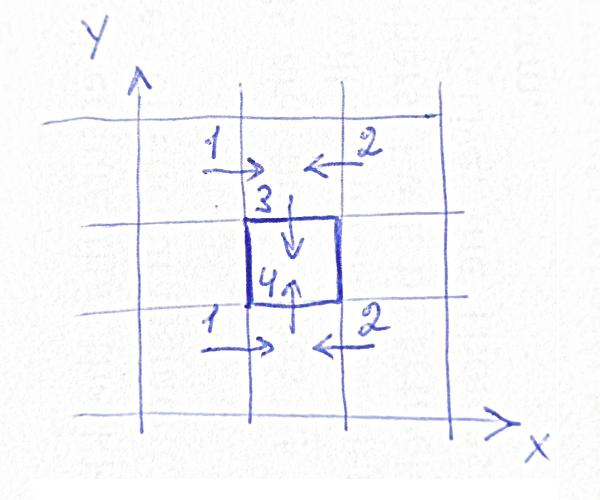
\includegraphics[width=.5\linewidth]{img/milestone08-domain-communication.jpg}
	\caption{Each process gets neighbor information without direct communication.}
	\label{fig:domain-communication}
\end{figure*}

This way it takes 6 steps instead of 26 for each process to get all information from its neighbors.

\subsection*{Stress estimation}

For the experiment with stretching a golden whisker we need to compute the reaction to strain --- the stress matrix.

\[
\sigma = \cfrac{1}{V} \sum_{i<j} \mat{r}_{ij} \times \mat{f}^T_{ij} = \cfrac{1}{V} \sum_i^{N} \sum_{j=i}^{N+N_G} \mat{r}_{ij} \times \mat{f}^T_{ij},
\]

where $\sigma\ (3, 3)$ - stress matrix for $xx, xy, \ldots zz$ directions, $V$ - total volume, $\mat{r}_{ij}\ (3, 1)$ - position, $\mat{f}^T_{ij}\ (1, 3)$ - force.

As we stretch the whisker in the $Z$ axis, I take only $\sigma(3, 3)$ value from this matrix (in experiments all other entries are near 0). The stress is per-atom, can be computed separately in each subdomain and then summed.



\clearpage

\section{Experiments}
\label{experiments}

Warning! Copying .xyz files in Meson didn't work for me, so I had to copy them to build directory by hand.

Code is structured in folders:
\begin{itemize}
	\item milestones --- CPP sources for simulation executables
	\item plot --- Python notebooks for plotting. Requires precomputed simultion results
	\item report --- the sources for the report you are reading now
	\item src --- common CPP files
	\item tests --- CPP tests using Google test framework
\end{itemize}

\subsection*{Velocity-Verlet test}

{\bf First test: constant acceleration.} For $m=1.0$, acceleration is equal to force. The movement distance under constant acceleration is well known: \[ S = v_0 t + \cfrac{at^2}{2} \]

I define two atoms:\\
first with position $r_1(1, 0, 0)$ and acceleration $a_1(1, 0, 0)$,\\
second with position $r_2(0, 1, 0)$ and acceleration $a_2(0, -0.5, 0)$.\\
Start velocity is 0 for simplicity. Following the formula, the resulting positions at $t = 10$ should be

\[ r_1(x, t=10) = 1 + 0 + \cfrac{1 \cdot 100}{2} = 51 \]
\[ r_2(y, t=10) = 1 + 0 - \cfrac{0.5 \cdot 100}{2} = -24 \]

The Verlet timestep in this test can be chosen as large as possible, the computed result always matches the analytical one.

{\bf Second test: linear acceleration.} I define acceleration as

\[ a(t) = 1 - t,\; t \in [0, 1] \]

Acceleration is derivative of velocity, so

\[ a = \cfrac{dv}{dt} \]

For a constant acceleration we use the well known formula \[ a = \frac{v_{end}-v_{start}}{t} \]

But for variable acceleration

\[ v(t) = \int_0^t a(t) dt + v_0 \]
\[ S(t) = \int_0^t v(t) dt \]
\[ S(t) = \int_0^t \left( \int_0^t a(t) dt + v_0 \right) dt\]

Now compute S using my definition of acceleration, with start velocity 0 for simplicity:

\[ v(t) = \int_0^t (1-t) dt = t - t^2 / 2\]
\[ S(t) = \int_0^t (t - t^2/2) dt = t^2/2 - t^3/6 \]

We obtained the analytical solution. Now define one atom with position $r(1, 0, 0)$. At $t=0.5$ its position should be

\[ r(x, t=0.5) = 1 + 0.5^2/2 - 0.5^3/6 = 1 + 5/(8 \cdot 6)\]

In this test the timestep must be small enough to capture the nonlinear changes in the velocity. I achieved approximate equality with $\Delta t = 0.00001$.

{\bf Implementation} --- src/atoms.h, src/verlet.cpp, src/verlet.h, tests/test\_verlet.cpp

\subsection*{First simulation}
In the first simulation, we don't care about physical units, and just set \( m=1, \sigma=1, \epsilon=1 \). Simulation duration is \( 100 \sqrt{m\sigma^2 / \epsilon} \), the atom positions are saved each \( 1 \sqrt{m\sigma^2 / \epsilon} \).  

Choice of the time step (multiplied by \( \sqrt{m\sigma^2 / \epsilon} \)):

\begin{enumerate}
	\item 0.05 or higher - immediate explosion
	\item 0.01 - already stable simulation, OVITO shows some atoms evaporate
	\item 0.001 or 0.0001 - similar result, drift in total energy is less than 0.01 eV. Some atoms still evaporate.
\end{enumerate}

The total energy was plotted for different time steps in Fig.~\ref{fig:first_simulation}.

{\bf Implementation}
\begin{lstlisting}[breaklines]
src/lj_direct_summation.cpp, 
src/lj_direct_summation.h,
tests/test_lj_direct_summation.cpp,
src/xyz.cpp,
src/xyz.h,
tests/test_verlet.cpp,
milestones/04/main.cpp
\end{lstlisting}


{\bf Plot} --- \verb|plot/energy_lineplot.ipynb|

\begin{figure*}[htb]
	\centering
	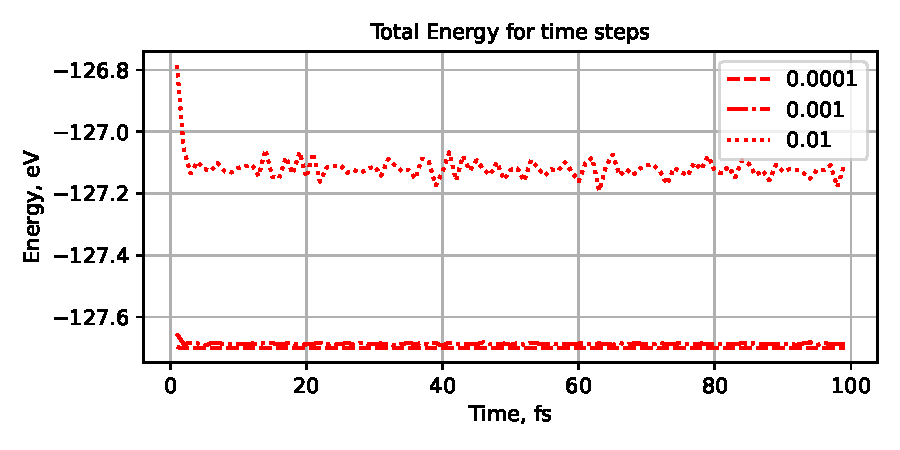
\includegraphics[width=.7\linewidth]{img/milestone04-total.pdf}
	\caption{With smaller step the simulation is more stable.}
	\label{fig:first_simulation}
\end{figure*}


\subsection*{Berendsen thermostat}

\begin{figure*}[htb]
	\centering
	\begin{minipage}{.3\textwidth}
		\centering
		\resizebox{\columnwidth}{!}{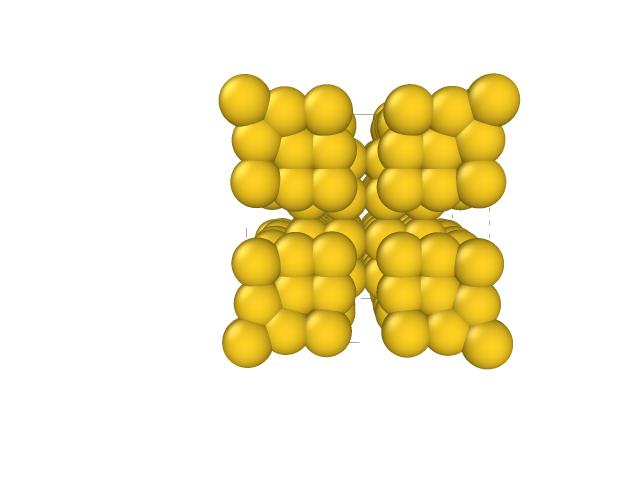
\includegraphics[trim={1.8cm 1.8cm 2.2cm 1.8cm},clip]{img/sim1.jpg}}
	\end{minipage}\hfill
	\begin{minipage}{.3\textwidth}
		\centering
		\resizebox{\columnwidth}{!}{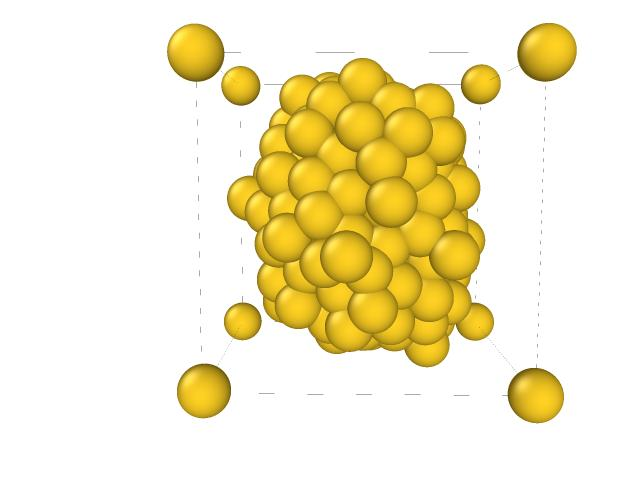
\includegraphics[trim={1.8cm 1.8cm 2.2cm 1cm},clip]{img/sim2.jpg}}
	\end{minipage}\hfill
	\begin{minipage}{.3\textwidth}
		\centering
		\resizebox{\columnwidth}{!}{
			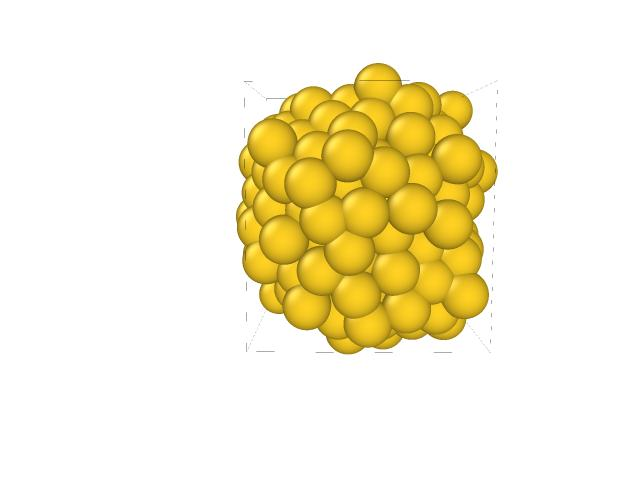
\includegraphics[trim={1.8cm 1.8cm 2.2cm 1cm},clip]{img/sim3.jpg}}
	\end{minipage}
	\caption{OVITO visualization of a cubic lattice with Berendsen thermostat. Without thermostat, atoms vaporize even with the smallest time step.}
	\label{fig:first_simulation_ovito}
\end{figure*}

I find that two aspects make the simulation successful: {\bf grid step} close to optimum of Lennard-Jones, and {\bf low target temperature} used in thermostat.

I create a cube of atoms of width 6 for this experiment, Fig.~\ref{fig:first_simulation_ovito}. The most stable configuration is where the grid step is $r = 2^{1/6}\sigma$, we know that to be the minimum of Lennard-Jones potential. Experiments with different $r$ behaved very badly.

At first I tried a high target temperature: 0.05 --- visualization shows that the atoms are pushed apart into infinity in small groups; 0.001 --- no vaporization. For this temperature, I choose Berendsen relaxation time (multiplied by \( \sqrt{m\sigma^2 / \epsilon} \)). Initially for $10$ time units I apply relaxation \( \tau_T = 1 \). Then for the whole simulation, \( \tau_T = 10 \) is required to keep the atoms from evaporating. 

In a second experiment I took a lower temperature $0.0001$. With this temperature it's enough to apply the thermostat only in the beginning for $10t$ with relaxation $\tau_T = 1$. After equilibration I can disable the thermostat and the system stays stable.

Testing the Berendsen implementation is very simple, because it modifies the speed of each atom separately, so it's enough to test the behaviour on just one atom. I tested that the temperature should exponentially approach the desired value, and in case the relaxation time is equal to \(\Delta t\), it should change instantly.

{\bf Implementation}
\begin{lstlisting}[breaklines]
src/lattice.cpp
src/lattice.h
src/thermostat.cpp
src/thermostat.h,
tests/test_thermostat.cpp
milestones/05/main.cpp
\end{lstlisting}


\subsection*{Neighbor list}

\begin{figure*}[htb]
	\centering
	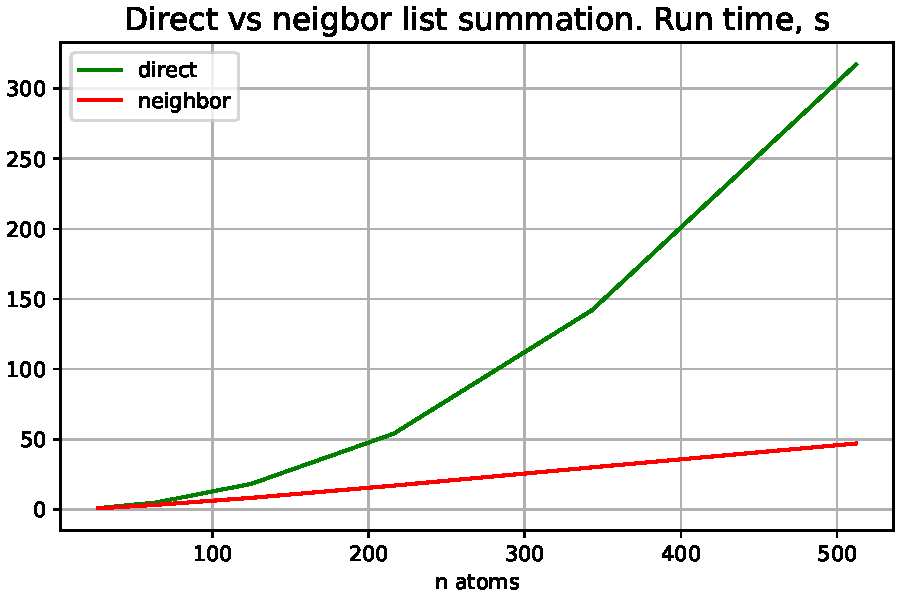
\includegraphics[width=.8\linewidth]{img/milestone06-time.pdf}
	\caption{Without neighbor list, time scales quadratically with number of atoms.}
	\label{fig:neighbor}
\end{figure*}

The provided implementation of neighbor lists is used. Cutoff radius is \( 3 \sigma \) to allow speedup, but not miss interactions. Execution time on clusters of different sizes is compared in Fig.~\ref{fig:neighbor} . Number of atoms: $3^3=27, 4^3=64, 5^3=125, 6^3=216, 7^3=343, 8^3=512$.

{\bf Implementation}
\begin{lstlisting}[breaklines]
src/neighbors.cpp,
src/neighbors.h,
tests/test_neighbors.cpp,
src/lj.cpp,
src/lj.h,
tests/test_thermostat.cpp
milestones/06/main.cpp
\end{lstlisting}

{\bf Run details}
\begin{itemize}
	\item Optimization level 3 must be enable before compilation.
	\item Run: \verb|cd buildDir/milestones/06; time ./milestone06 [n]|
	\item Plot with \verb|plot/time_lineplot.ipynb|
\end{itemize}

\subsection*{Heating experiment}

{\bf Equilibration} with Berendsen thermostat is done for the first 100 fs with $\tau_T$ = 100 fs and target temperature 300 K = 27 C.

With correct force recomputation, even a large time step $\Delta t=10$ fs causes total energy drift no more than 1 eV in 100 000 fs (without thermostat and heat deposition), we can safely use it for this simulation. Before the error was fixed, it drifted no matter which $\Delta t$ I chose. Now I disable the thermostat after equilibration for fair energy measurements. Smaller $\Delta t = 1$ fs showed similar results. The intuition for choosing the time step is, that it must be much smaller than oscillation period of an atom. The gold atoms have large mass thus a large step is acceptable. One oscillation takes around 1000 fs.

Simulation parameters:
\begin{itemize}
	\item total = 100 000 fs
	\item step $\Delta t$ = 10 fs
	\item deposit interval = 4000 fs
	\item print interval = 1000 fs
\end{itemize}

The heat deposited in each interval was $\Delta Q$ = 20 eV, 100 eV, and 200 eV for small Mackay cluster, big Mackay cluster and the whisker respectively.

\subsubsection*{Adding heat}

To add a fixed amount of energy $Q$ we scale the velocities by $\lambda$:

\[
\begin{aligned}
	E_k &= \frac{1}{2} \sum_i m v_i^2 \\
	E_k + Q &= \frac{1}{2} \sum_i m (\lambda v_i)^2 = \lambda^2 \frac{1}{2} \sum_i m v_i^2 \\
	E_k + Q &= \lambda^2 E_k \\
	\lambda^2 &= 1 + \frac{Q}{E_k} \\
\end{aligned}
\]

{\centering\framed{ \( \lambda = \sqrt{1 + \frac{Q}{E_k}} \) }\\}

{\bf Latent heat} is the energy to transform from solid to liquid state. During melting the temperature stays the same, but potential energy increases. {\bf Heat capacity} is the coefficient $dE/dT$ of linear relation between $E_{tot}$ and $T$ (without thermostat it actually becomes linear).

I simulated the Makay-923 and Makay-3871 Makay clusters, introduced in \cite{MakayOriginal} and implemented by Dr Lars Pastewka in \cite{MakayPastewka} and generated Whisker-6950 using the \verb|make_whisker.py| script.
As the simulation doesn't have truly constant melting temperature, I took the middle point between linear regions on the energy-temperature plot (Fig.~\ref{fig:heat-makay1},~\ref{fig:heat-makay2},~\ref{fig:heat-whisker}). To measure the heat capacity coefficient I take two faraway points on the energy-temperature plot and compute $(E_2-E_1)/(T_2-T_1)$. To measure latent heat I extrapolate the lines for solid phase and liquid phase to the assumed melting point and take the difference in energies (Fig.~\ref{fig:heat-estimated}).

\begin{figure*}[h!]
	\centering
	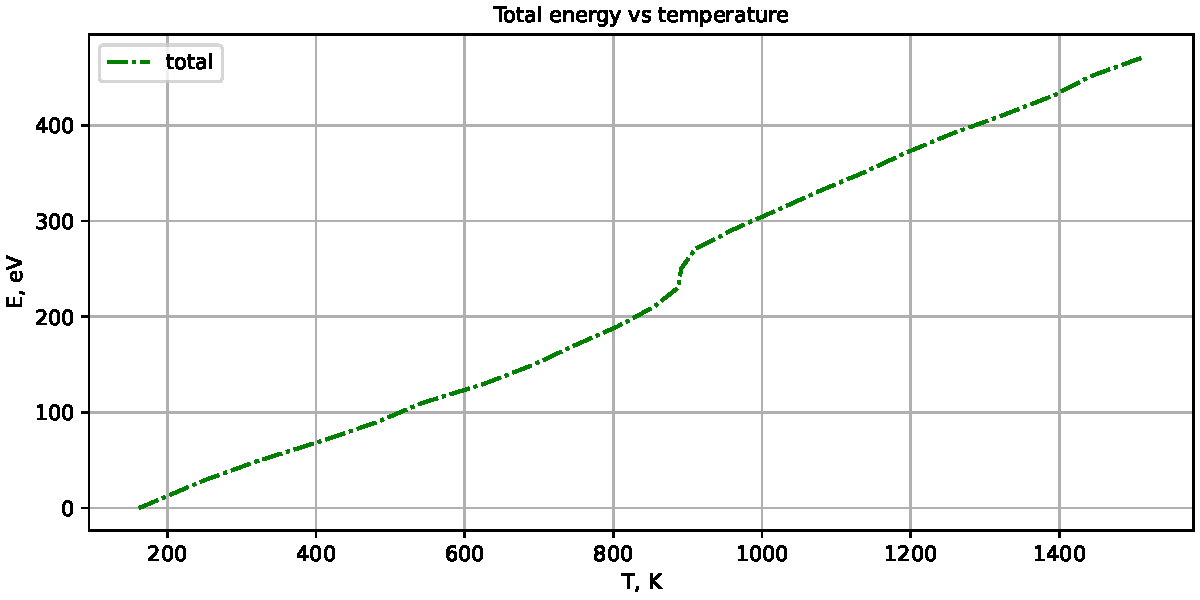
\includegraphics[width=.8\linewidth]{img/milestone07-small.pdf}
	\caption{Total energy (eV) vs temperature (K) for Makay-923.}
	\label{fig:heat-makay1}
\end{figure*}

\begin{figure*}[h!]
	\centering
	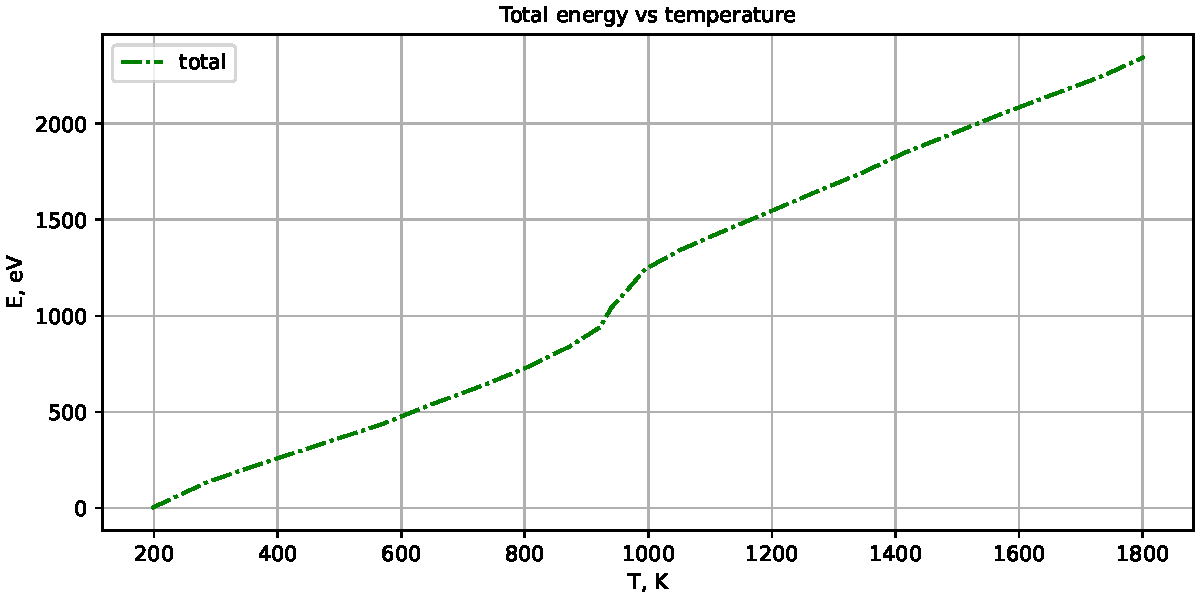
\includegraphics[width=.95\linewidth]{img/milestone07-large.pdf}
	\caption{Total energy (eV) vs temperature (K) for Makay-3871.}
	\label{fig:heat-makay2}
\end{figure*}

\begin{figure*}[h!]
	\centering
	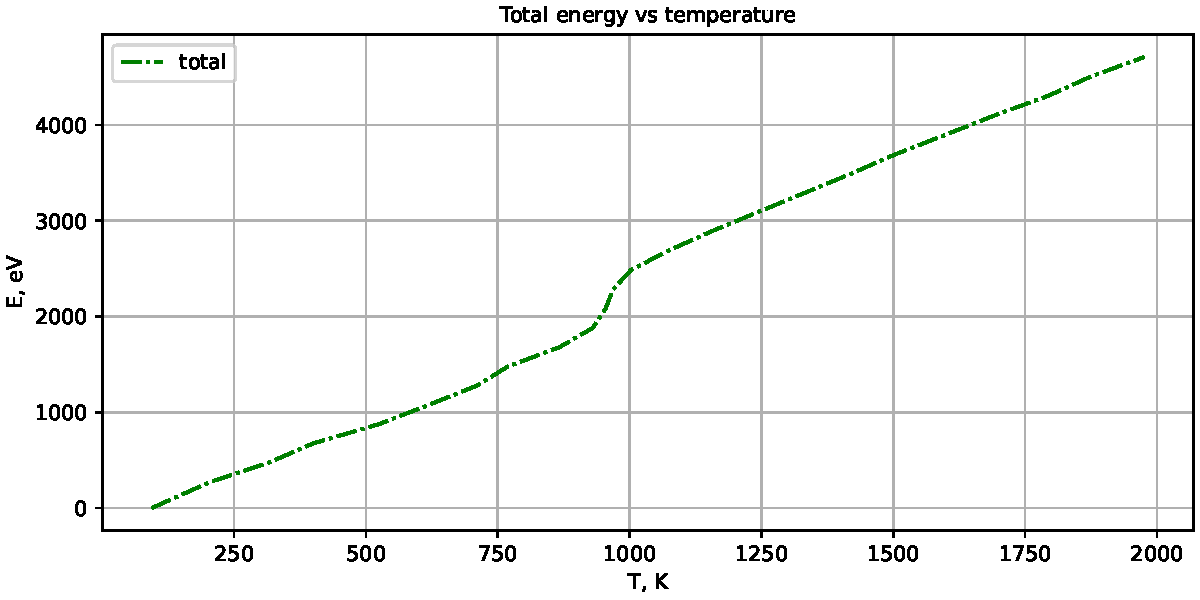
\includegraphics[width=.95\linewidth]{img/milestone07-whisker.pdf}
	\caption{Total energy (eV) vs temperature (K) for Whisker-6950.}
	\label{fig:heat-whisker}
\end{figure*}

\begin{figure*}[h!]
	\centering
	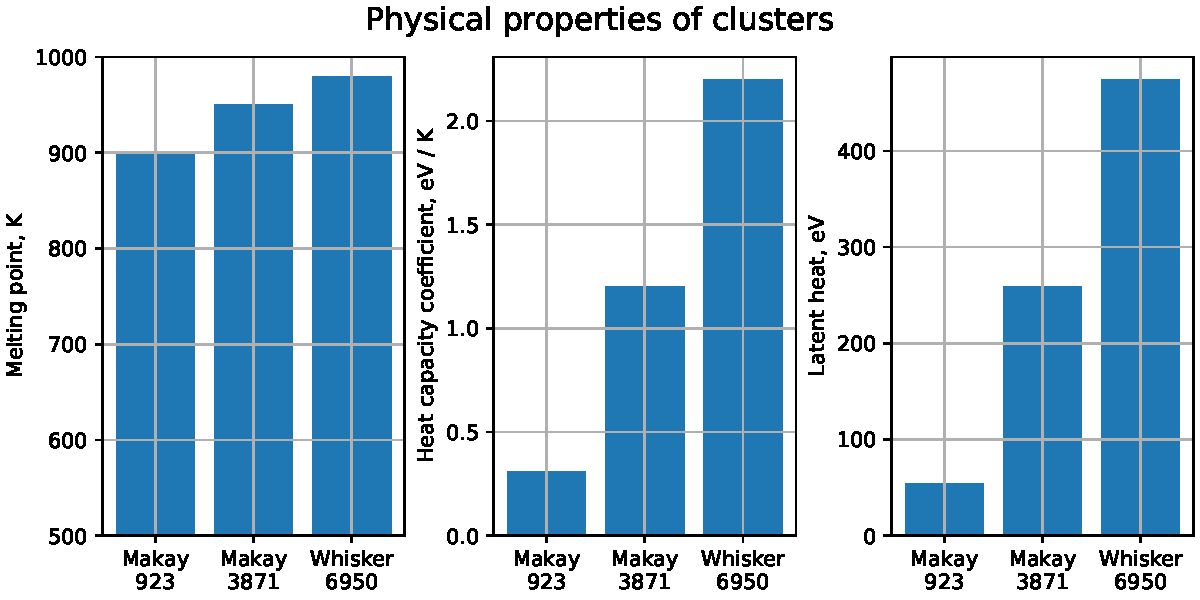
\includegraphics[width=.9\linewidth]{img/milestone07-bar.pdf}
	\caption{Estimated Melting point (K), Heat capacity coefficient, Latent heat (eV) for each cluster.}
	\label{fig:heat-estimated}
\end{figure*}

\newpage

{\bf Implementation}
\begin{lstlisting}[breaklines]
src/ducastelle.h,
src/ducastelle.cpp,
milestones/07/main.cpp
\end{lstlisting}

{\bf Run details}
\begin{itemize}
	\item Outputs are generated in \verb|buildDir/milestones/07|
	\item Plot with \verb|plot/milestone07.ipynb|
\end{itemize}

\newpage

\subsection*{Parallelization}

I used the gold cluster Mackay-3871. With $\Delta t$ = 10 fs, total energy fluctuates no more than 0.5 eV in 10 000 fs, simulation for 100 000 fs didn't show larger fluctuation. Also, the temperature plot shows that atom oscillation has a period of around 1000 fs, it confirms that this step size is reasonable (Fig.~\ref{fig:parallel-1},~\ref{fig:parallel-2},~\ref{fig:parallel-3})

One cause of instability was that atoms on the domain edge disappeared. Solution: add offset to atom positions, so that they don't drop out from the simulation domain.

{\bf Run details}
\begin{itemize}
	\item Edit source code, set domain to (1, 2, 2)
	\item \verb|mpirun -n 4 --oversubscribe ./milestone08|
	\item Outputs are generated in \verb|buildDir/milestones/08|
	\item Plot with \verb|plot/milestone08.ipynb|
\end{itemize}

\begin{figure*}[h!]
	\centering
	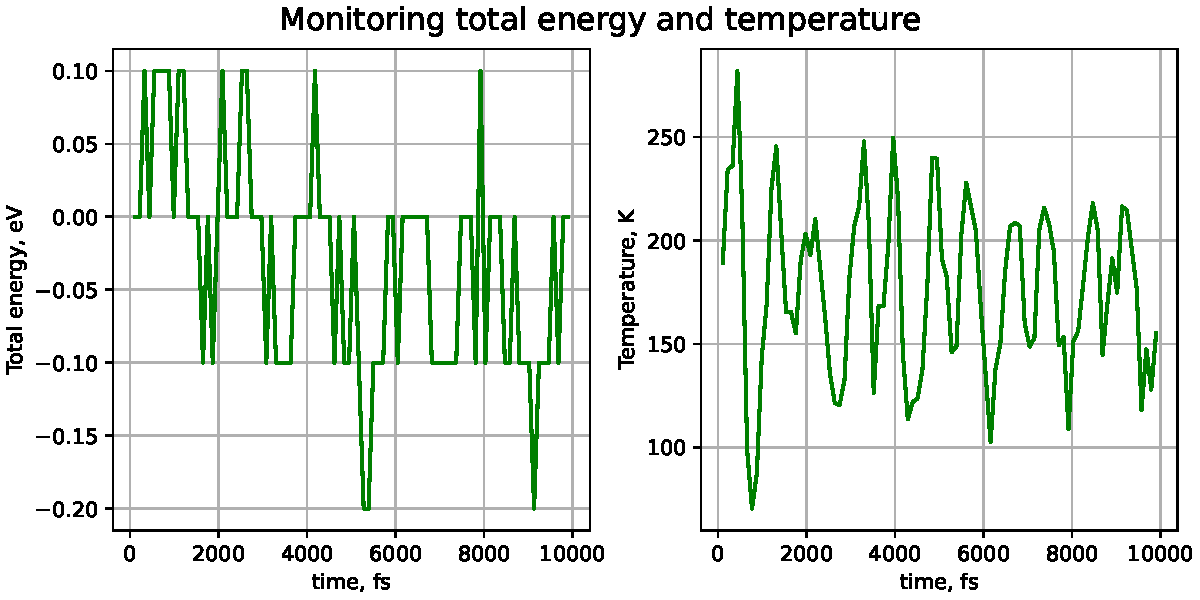
\includegraphics[width=.8\linewidth]{img/milestone08-1proc.pdf}
	\caption{Parallelized with 1 process.}
	\label{fig:parallel-1}
\end{figure*}

\begin{figure*}[h!]
	\centering
	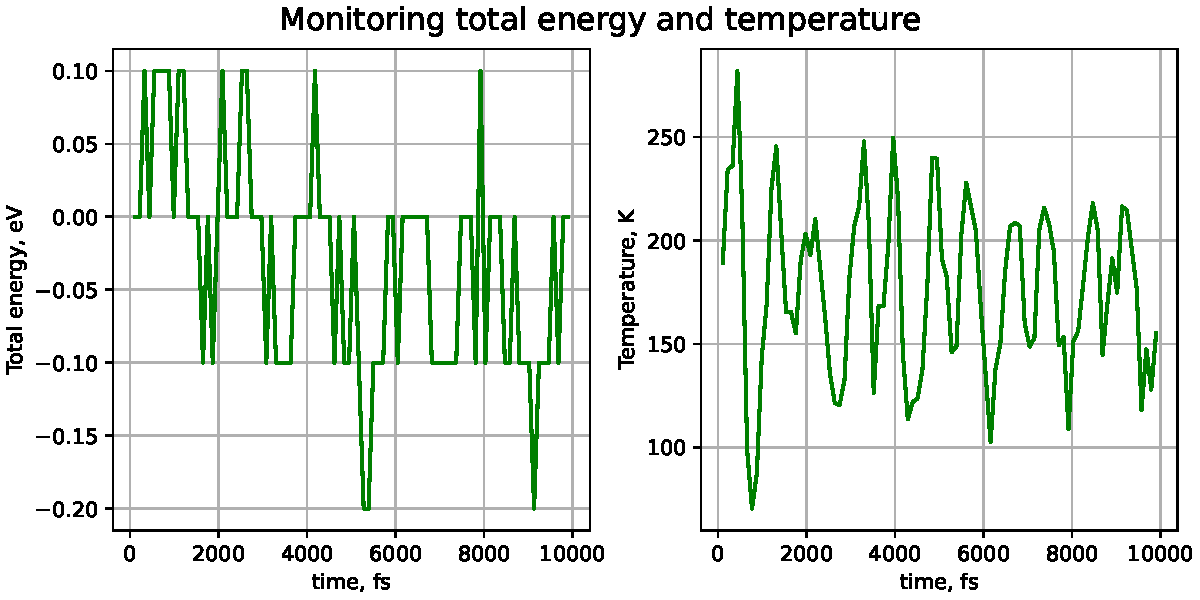
\includegraphics[width=.85\linewidth]{img/milestone08-4proc.pdf}
	\caption{Parallelized with 4 processes.}
	\label{fig:parallel-2}
\end{figure*}

\begin{figure*}[h!]
	\centering
	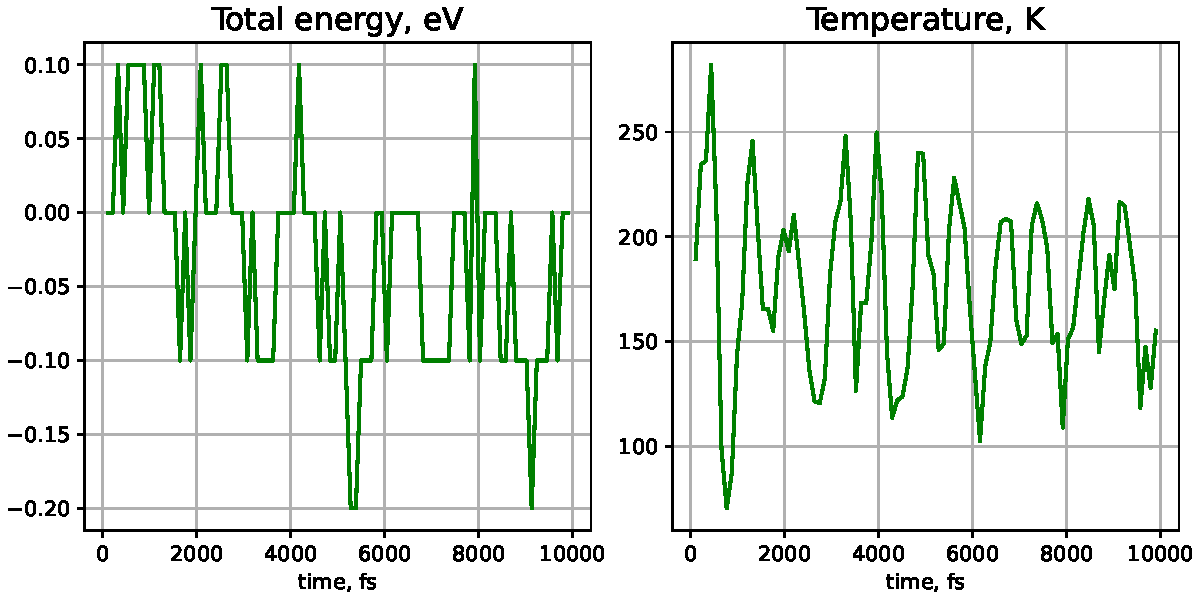
\includegraphics[width=.85\linewidth]{img/milestone08-8proc.pdf}
	\caption{Parallelized with 8 processes.}
	\label{fig:parallel-3}
\end{figure*}

{\bf Implementation}
\begin{lstlisting}[breaklines]
src/mpi_support.h
src/domain.h
src/domain.cpp
milestones/08/main.cpp
\end{lstlisting}

\clearpage % works for figures too!

\subsection*{Pulling a gold nanowire}

Here we use a gold rod with periodicity along Z axis. The distance between the end and the periodical beginning of the rod must be on the order of potential optimum, otherwise the system will explode or be disconnected. I equilibrate the temperature using Berendsen thermostat in the beginning of simulation. After that domain scaling along Z axis is applied, which causes strain inside the material.

I used temperatures 300 and 500 K; deformation length 10 and 20 angstrem. Total duration was 100 000 fs which causes a deformation of $10^{-4}$ A/fs in the first case.

We observe the measured stress force over strain (Fig.~\ref{fig:whisker-300},~\ref{fig:whisker-500}). The stress force was averaged over 5000 fs which allows us to see the clear pattern of defect formation.

For the 300 K room temperature, the faster elongation breaks the wire more significantly, because stress drops much more and doesn't recover with time. The temperature is low, thus the material is more brittle.

For 500 K the situation is much different. Firstly, the stress changes more slowly, the material starts regrouping on lower values of stress (strain=10 A, at t=300 K max=0.0045, while at t=500 K max=0.0035) and also recovers better. Especially for the fast stretching, the rod completely broke only at the end. It looks like with higher temperature the material can flow more freely, but still forms regular solid-like structures locally. That explains that the stress doesn't go completely down.

For visualization of defects I found slice operation in OVITO and used Common Neighbor Analysis (Fig.~\ref{fig:whisker-defect}). The atoms have shifted, but preserve the local grid structure, which is natural for low temperatures.

\begin{figure*}[h!]
	\centering
	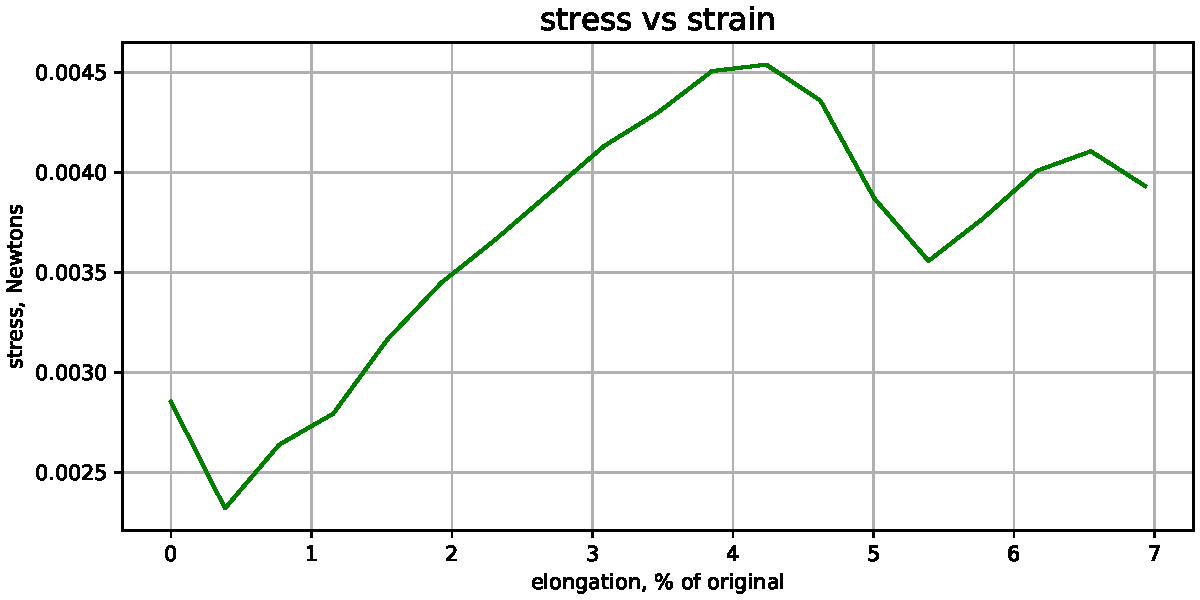
\includegraphics[width=.85\linewidth]{img/milestone09-small-300-10.pdf}
	\caption{Small whisker, 300 K, elongation by 10 A.}
	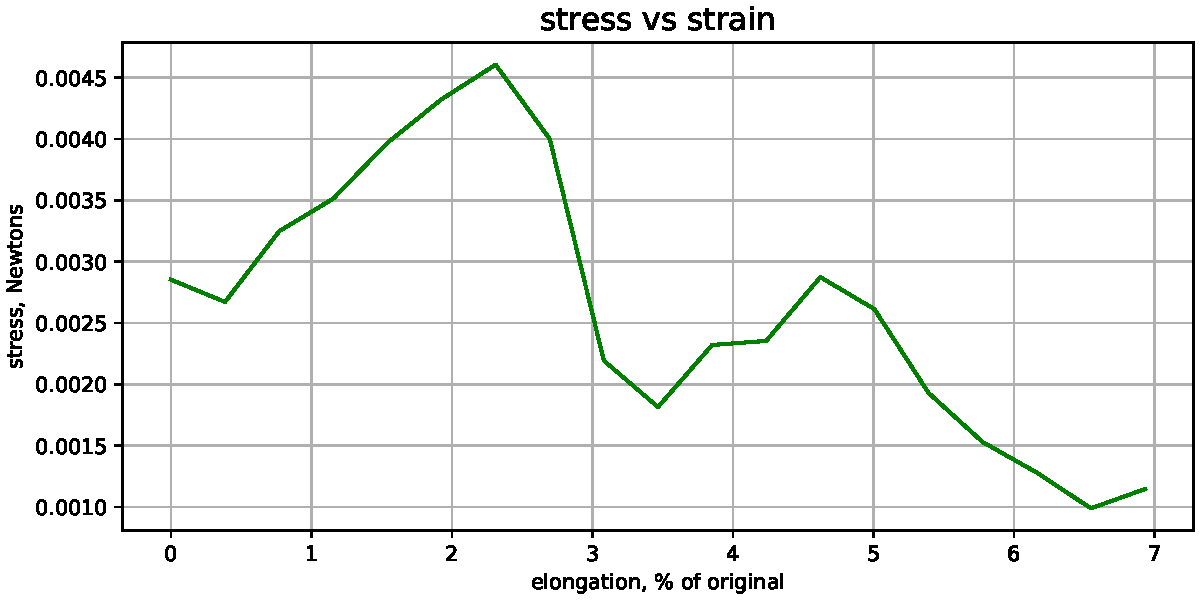
\includegraphics[width=.85\linewidth]{img/milestone09-small-300-20.pdf}
	\caption{Small whisker, 300 K, elongation by 20 A.}
	\label{fig:whisker-300}
\end{figure*}

\begin{figure*}[h!]
	\centering
	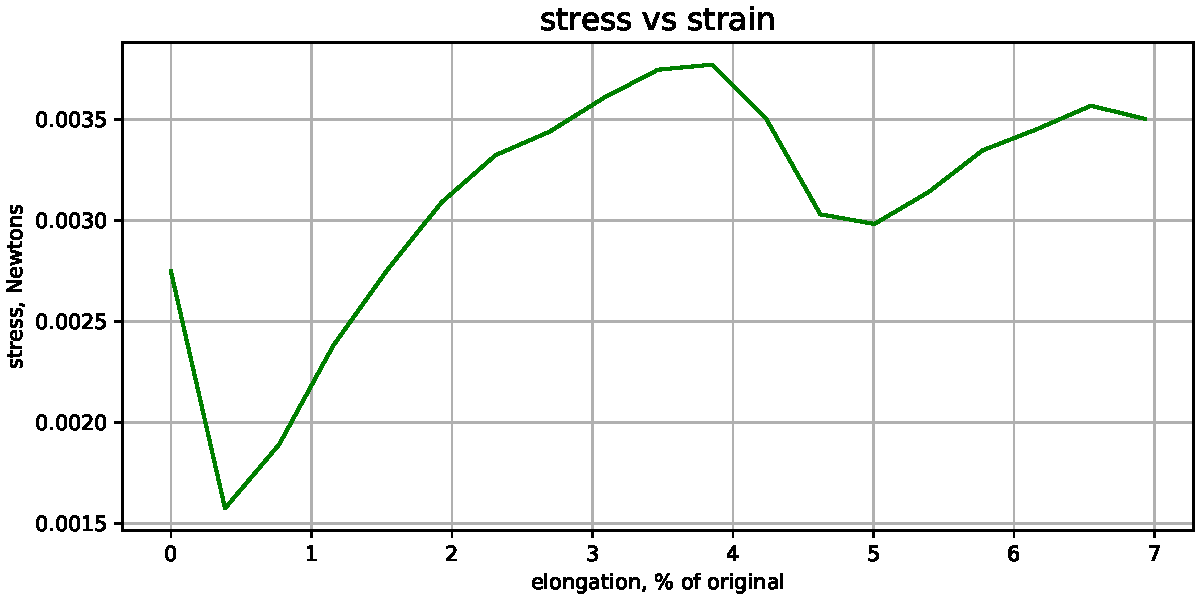
\includegraphics[width=.85\linewidth]{img/milestone09-small-500-10.pdf}
	\caption{Small whisker, 500 K, elongation by 10 A.}
	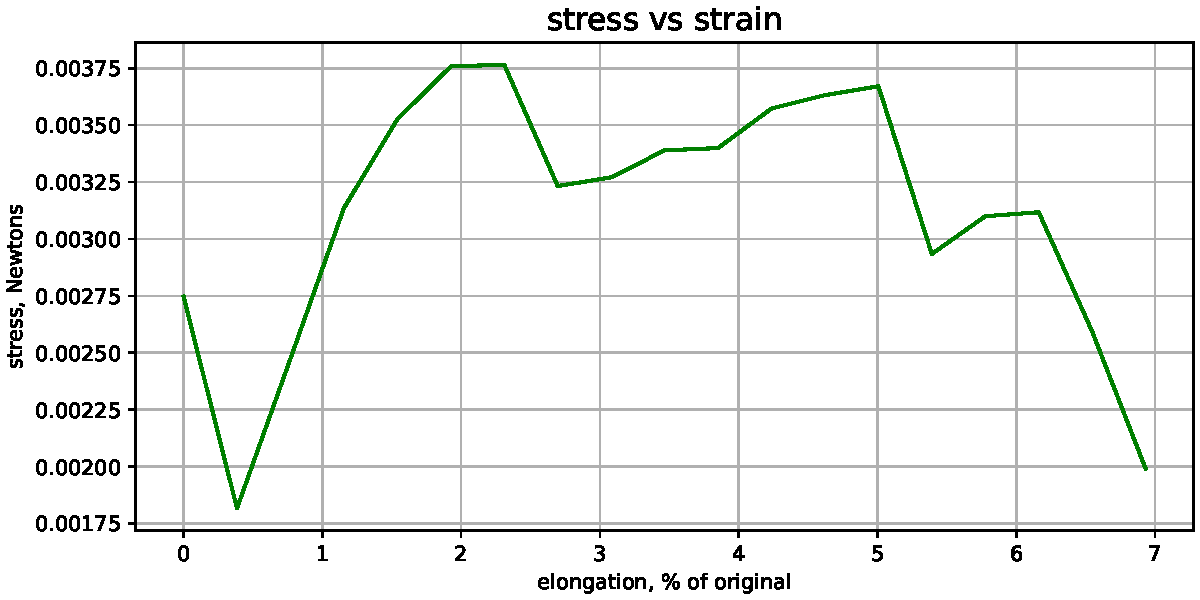
\includegraphics[width=.85\linewidth]{img/milestone09-small-500-20.pdf}
	\caption{Small whisker, 500 K, elongation by 20 A.}
	\label{fig:whisker-500}
\end{figure*}

\begin{figure*}[h!]
	\centering
	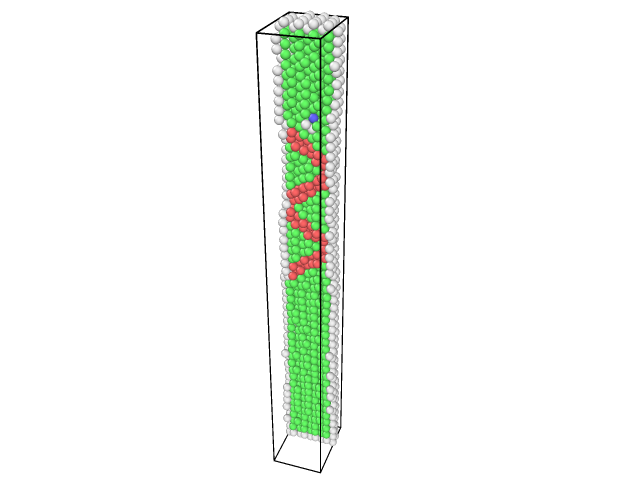
\includegraphics[width=.85\linewidth]{img/milestone09-small-300-10-pic.png}
	\caption{Small whisker, 300 K, elongation by 10 A. The rod is sliced in half, in red we see the break point.}
	\label{fig:whisker-defect}
\end{figure*}


{\bf Run details}
\begin{lstlisting}[breaklines]
cd buildDir/milestones/09
mpirun -n 4 --oversubscribe ./milestone09 300.0 10 whisker_small.xyz 1
sbatch run.job ./buildDir/milestones/09/milestone09 300.0 10.0 whisker_small.xyz 1
\end{lstlisting}

Domain decomposition is done automatically based on available number of processes.
For some reason the big whisker fails to run with an error in neighbors "neighbor list not yet computed".

{\bf Implementation}
\begin{lstlisting}[breaklines]
milestones/09/main.cpp
\end{lstlisting}

\clearpage
\section{Conclusion}
\label{conclusion}

In this report I implemented a program that is capable of running a Molecular Dynamics simulation in parallel on a cluster. The report covers efficient implementation of the simulation using neighbor lists for the interatomic potentials, parallelization for multiple CPUs. The characteristics of materials were measured: energy of system, melting point, latent heat, heat capacity, stress force.

\newpage
{\small
	\bibliographystyle{plain}
	\bibliography{egbib}
}

\end{document}
